\documentclass[pdf]{planckDoc}
\usepackage{alltt}
\usepackage{verbatim}

\sloppy

\begin{document}

\renewcommand{\d}{\mathrm{d}}
\newcommand{\tw}[1]{\texttt{#1}}

\title{Compilation and Usage of the Planck Simulation Modules}
\author{Martin Reinecke, Klaus Dolag}
\authorised{no one}
\date{\today}
\docid{PL-COM-MPA-MA-SIM007}
\docrv{unknown}
\abstract{This document summarises how the modules for Planck data
simulation can be compiled and used.}

\frontpage

\section{Simulation Code}

\subsection{Obtaining the code}

The simulation packages reside in the IDIS CVS respository
at ESTEC. If you do not know how to get there, contact Martin Bremer
(\tw{mbremer@rssd.esa.int}) for \tw{<username>}
and the related password.

{\bf Note:} It is not recommended to copy a CVS file tree from someone else,
because CVS remembers the user who did the original checkout in the
{\tt */CVS/Root} files. That means that the user who copied the files
will not be able to update them or commit changes.

To do an initial checkout of the LevelS sources you should issue the
following commands:
 \begin{verbatim}
 setenv CVSROOT :pserver:<username>@cvs.rssd.esa.int:/services/repositories/PLANCK_CVS
 (or export CVSROOT=:pserver:<username>@cvs.rssd.esa.int:/services/repositories/PLANCK_CVS)
 cvs login
 cvs co -P planck/LevelS
 \end{verbatim}

Please note that the local directory {\tt planck/LevelS} should not exist
before the checkout.

\subsection{Updating your version of the code}

To update your copy of the source code, enter the directory \tw{planck/LevelS}
and issue the command
\begin{verbatim}
cvs -q update -Pd
\end{verbatim}

\subsection{Compilation}

In order to compile the code you will need following programs:
\begin{itemize}
   \item an up-to-date version of \tw{GNU make}. Parallel compilation is
     supported for \tw{GNU make} 3.79 and later.
   \item a \tw{C} compiler supporting the C90 standard.
   \item a \tw{C++} compiler supporting the C++98 standard; this includes
     \tw{g++} 3.0 and above and the compilers of SGI and IBM.
   \item a Fortran 95 compiler with support for the Fortran 2003 module
     \tw{iso\_c\_binding}. This includes \tw{GNU gfortran} 4.3 and above as well
     as Intel \tw{ifort} 10.0 and above.
\end{itemize}
To compile the code, follow the instructions
in \tw{planck/LevelS/README.compilation}.

Note: in order to make use of hybrid C++/Fortran modules, it is required that
the employed C++ and Fortran compilers come from the same ``vendor'', like
\tw{g++/gfortran} or \tw{icpc/ifort}.

\clearpage
\section{Test Pipeline}

\begin{itemize}

\item To run the simulation, you will need the following items:
   \begin{itemize}
   \item Template maps and beam patterns. \\
      In order to keep code and data separate, there are no template maps,
      spectra or beam patterns included in the package.
      An archive file containing all the data necessary for the test
      pipeline can be downloaded from MPA's Planck web pages at\\
      \href{http://planck.MPA-Garching.MPG.DE/SimData/test/testdata.tar.gz}
        {http://planck.MPA-Garching.MPG.DE/SimData/test/testdata.tar.gz}.
   \item \tw{xv} \\
      The image viewer \tw{xv} is used only for displaying some
      results. It is thus not strictly required.
      If you prefer another image viewer, you can enter its name when
      \tw{SetupSimulation} asks for it.
   \end{itemize}

\item Run the setup script \tw{planck/LevelS/SetupSimulation}.
It will ask for the path containing the template data and module binaries,
the name of your image viewer and several other simulation-specific
parameters which are explained in chapter \ref{simparam}.

\item The script creates the parameter files necessary for running the test
pipeline and tells you how to start the simulation.

If everything worked fine, the image viewer will show you
the results of your test run. You can compare them with our sample run
available on our web pages at\\
\href{http://planck.MPA-Garching.MPG.DE/SimData/index_test.html}
{http://planck.MPA-Garching.MPG.DE/SimData/index\_test.html}.

\item Be aware that the \tw{Pipeline} script only offers
a way for testing your self-compiled simulation packages and
is thus only a very specialized simulation. If you want to produce
\emph{real} data, you need to set the parameters of each step carefully
according to the requirements of the simulation you want to run.

\end{itemize}

\clearpage
\section{Simulation parameters}
\label{simparam}

\begin{itemize}

\item \tw{NSIDE}

The resolution of the output maps produced by the pipeline
(i.e.~the \tw{HEALPix NSIDE} parameter).
It has to be a power of 2 and should lie between 16 and 512.

The sky is tesselated into $12\,N_\mathrm{side}^2$ pixels. This implies
that the approximate side length of a HEALPix pixel is
$$
  \delta\theta\approx\sqrt{\frac{3}{\pi}}\,
  \frac{3600}{N_\mathrm{side}}\;\hbox{arc minutes}\;.
$$
This gives a clue for the choice of $N_\mathrm{side}$ required by
your simulation.

\item \tw{LMAX}

This quantity determines how accurately the ``synthetic skies'' are
calculated, which are scanned by the detector later on.
The \tw{LMAX} parameter should be twice to three times the value chosen
for \tw{NSIDE}, up to a maximum of 2900. Note that the foreground maps
distributed in \tw{testdata.tar.gz} only contain $a_{lm}$ up to
$l_{\mathrm{max}}=1024$, so that a higher $l$ will not further improve the
quality of the foreground signal.

\item Detector name

Depending on this, all characteristic quantities like detector frequency,
sampling frequency, bandwidth, noise amplitudes, orientation relative to
the optical axis etc.\ are determined from the focal plane database.
If a simulation with special parameters is required, an additional detector
with the desired parameters has to be added by hand to the database.

\item First and last pointing period of the mission

These parameters influence the sky coverage of the simulation and also the
size of the output files. If unsure, leave them at the default of -1, which
means that all pointing periods available in the input PPL file will be used.

\item Nominal vs.\ realistic pointing

If realistic pointing is chosen, detailed pointing information with
synthesised pointing errors is created for each pointing period, and
the sky is scanned 60 times instead of once per period.
This will increase the overall running time by roughly a factor of 60
and also require more storage space for intermediate data.

\end{itemize}

\clearpage
\section{The Simulation Package}
%---------------------------------------------------------------------
%---------------------------------------------------------------------
%---------------- Libraries ------------------------------------------
%---------------------------------------------------------------------
%---------------------------------------------------------------------
\subsection{Libraries}

\subsubsection{cfitsio}

The cfitsio library can be obtained from
\href{http://heasarc.gsfc.nasa.gov/docs/software/fitsio/fitsio.html}
{http://heasarc.gsfc.nasa.gov/docs/software/fitsio/fitsio.html}.
LevelS currently uses version 3.35.

\subsection{Optional external packages}
  \subsubsection{fv}
      You may want to install the interactive FITS file viewer
      \tw{fv}, which can be obtained from
      \href{http://heasarc.gsfc.nasa.gov/docs/software/ftools/fv}{HEASARC}.
      It is very convenient for looking at the data in FITS files, plotting
      them or making images from them. It can also be used for editing
      header information.


%---------------------------------------------------------------------
%---------------------------------------------------------------------
%---------------- Simulation Modules ---------------------------------
%---------------------------------------------------------------------
%---------------------------------------------------------------------
\subsection{Module descriptions}
\textbf{Note to the authors of the simulation modules}\\
We have tried our
best in extracting the overviews and the descriptions of the
parameters from the documentation provided in your packages. If there
are errors in this text, or if you would like to give a more detailed
description of your modules or their parameters, please send any
comments to Martin Reinecke (\tw{martin@mpa-garching.mpg.de}), who
will be happy to add them to this document.

\vspace{0.3cm}

\textbf{Parameter file format}\\
The modules read parameters from ASCII files. Each parameter is
defined in a separate line of the form:
\begin{verbatim}
[name] = [value]
\end{verbatim}
Lines starting with a \tw{\#} sign are ignored and can thus be
used as comment lines.

\subsubsection{CAMB}

(A.~Lewis \& A.~Challinor)

\href{http://camb.info}{http://camb.info}

\begin{alltt}
camb [parameter file]

example parameter file:

\input{../CAMB/camb.par.txt}
\end{alltt}

%---------------------------------------------------------------------
%---------------- HEALPix --------------------------------------------
%---------------------------------------------------------------------

\subsubsection{HEALPix}

(K.~G\'orski, E.~Hivon, B.~Wandelt, A.J.~Banday, M.~Bartelmann, M.~Reinecke)

This is a software package for HEALPix
(\href{http://healpix.sourceforge.net}{http://healpix.sourceforge.net}),
the Hierarchical, Equal Area, and
iso-Latitude Pixelisation of the sphere, which was originally devised
in early 1997 by Krzysztof M.~G\'orski at the Theoretical Astrophysics
Center in Copenhagen. Early development of the HEALPix concept and
initial implementation was made in the spring of 1997 in collaborative
work of K.~G\'orski with Eric F.~Hivon, currently at Caltech. Benjamin
D.~Wandelt, currently at Princeton, has contributed critically to the
further development of HEALPix and related mathematical methods.

\begin{itemize}

\item \tw{syn\_alm\_cxx}:
Given a power spectrum, this program produces a Gaussian realisation of this
power spectrum in the form of spherical harmonic coefficients.
These coefficients can be further processed by \tw{alm2map\_cxx}.

\begin{alltt}
syn\_alm\_cxx [parameter file]

\input{../Healpix_cxx/syn_alm_cxx.par.txt}
\end{alltt}

\item \tw{alm2map\_cxx}: This program can be used to create HEALPix
maps (temperature only or temperature and polarisation)
from $a_{\ell m}$ coefficients. Total operation count
scales as ${\cal O}(N_{\rm pix}^{3/2} \log{N_{\rm pix}})$ with a
prefactor dependent on the limiting spherical harmonics order
$\ell_{\rm max}$ of the actual problem.  The map resolution, Gaussian beam
FWHM, and random seed for the simulation can be selected by the user.

\begin{alltt}
alm2map_cxx [parameter file]

\input{../Healpix_cxx/alm2map_cxx.par.txt}
\end{alltt}

\item \tw{anafast\_cxx}: This program performs harmonic analysis of the
HEALPix maps up to a user specified maximum spherical harmonic order
$\ell_{max}$.
%  The integrals are computed on the whole sphere, unless
%the user chooses a provided option to excise from the input map(s) a
%simple, constant latitude, galactic cut.
Scalar, or scalar and
tensor, spherical harmonic coefficients are evaluated from the map(s)
if the input provides, respectively, only the temperature, or
temperature and polarisation maps.  The total operation count scales
as ${\cal O}(\sqrt{N_{\rm pix}} l_{\rm max}^2)$ with a prefactor
depending on $\ell_{max}$.

\tw{anafast\_cxx} reads a file containing the map(s) and produces a file
containing the temperature power spectrum $C^T_l$ and, if requested,
also the polarisation power spectra $C^E_l$, $C^B_l$ and $C^{T\times
E}_l$.  The $a_{lm}$ coefficients computed during the execution also
can be written to a file if requested.

\tw{anafast\_cxx} executes an approximate, discrete point-set quadrature on a
sphere sampled at the HEALPix pixel centers.  Spherical harmonic
transforms are computed using recurrence relations for Legendre
polynomials on co-latitude, $\theta$, and Fast Fourier Transforms on
longitude, $\phi$.

\tw{anafast\_cxx} permits two execution options which allow a significant
improvement of accuracy of the approximate quadrature performed by
this facility:

\begin{itemize}

\item An improved analysis using the provided ring weights, which
correct the quadrature on latitude, and/or

\item An iterative scheme using in succession several backward and
forward harmonic transforms of the maps.

\end{itemize}

\begin{alltt}
anafast_cxx [parameter file]

\input{../Healpix_cxx/anafast_cxx.par.txt}
\end{alltt}

\item \tw{map2tga}: This facility provides a means to
generate a TGA image from an input HEALPix sky map. It is intended to
allow some primitive visualisation for those with limited or no access
to IDL.  It is also useful for image generation in a pipeline
environment. \tw{map2tga} can read parameters from the command line or
from a file.

\begin{alltt}
\input{../Healpix_cxx/map2tga.par.txt}
\end{alltt}

\item \tw{rotalm\_cxx}: Converts $a_{lm}$ between different coordinate systems.

\begin{verbatim}
Usage: rotalm_cxx <infile> <outfile> <itransform> <pol>
or   : rotalm_cxx <infile> <outfile> <psi> <theta> <phi> <pol>

itransform: 1: Equatorial (2000) -> Galactic   (2000)
            2: Galactic   (2000) -> Equatorial (2000)
            3: Equatorial (2000) -> Ecliptic   (2000)
            4: Ecliptic   (2000) -> Equatorial (2000)
            5: Ecliptic   (2000) -> Galactic   (2000)
            6: Galactic   (2000) -> Ecliptic   (2000)
            7: Equatorial (1950) -> Galactic   (1950)
            8: Galactic   (1950) -> Equatorial (1950)
            9: Equatorial (1950) -> Ecliptic   (1950)
           10: Ecliptic   (1950) -> Equatorial (1950)
           11: Ecliptic   (1950) -> Galactic   (1950)
           12: Galactic   (1950) -> Ecliptic   (1950)

psi, theta, phi: Euler angles (in degrees)

pol: T or F
\end{verbatim}
\end{itemize}

\subsubsection{Almmixer}
\label{almmix}

(Martin Reinecke, MPA)

This module reads CMB temperature fluctuation $a_{lm}$ and various
foreground $a_{lm}$, calculates the frequency-dependent intensities of all
contributions and convolves them with the response function $W_\nu$ of
a given detector. The resulting combined set of $a_{lm}$ is written in units of
antenna temperature.

The antenna temperature $T_\mathrm{A}$ is defined as follows:

\begin{equation}
T_\mathrm{A} = \int \frac{d T_\mathrm{A}(\nu)}{d \nu}  d \nu
    = \int \frac{W_\nu c^2}{2 \nu^2 k} \frac{d F(\nu)}{d \nu} d \nu
\end{equation}

This quantity is calculated approximately by subdividing the frequency band
of the detector into many sub-bands, computing the contribution of the $n$th
sub-band using the formula
\begin{equation}
{T_\mathrm{A}}_n = \frac{{W_\nu}_n c^2}{2 \nu_n^2 k}
                   \frac{d F(\nu_n)}{d \nu}\, \Delta\nu_n,
\end{equation}
where $\nu_n$ is the central frequency of the sub-band, and $\Delta\nu_n$ is its
width, and summing over all ${T_\mathrm{A}}_n$.

So far, \tw{almmixer} knows about the following radiation sources:
\begin{itemize}
 \item CMB (from \tw{synfast}):\\
   Thermodynamic temperature fluctuations in Kelvin. This information is used
   to determine the spectral intensity at the required frequencies.
 \item Galactic dust emission:\\
   Input is given at 100$\,\mu$m in MJy/sr and extrapolated to the actual
   frequency using the spectrum shown in the left panel of Fig.~\ref{spec}.
   The dust temperature can be adjusted.
 \item Galactic dust emission with a simplified 2-component model:\\
   Input is given at 100$\,\mu$m in MJy/sr and extrapolated to the actual
   frequency using a 2-component model suggested by C.~Baccigalupi.
 \item Galactic synchrotron emission:\\
   Input is given at 408$\,$MHz in MJy/sr and extrapolated to the actual
   frequency using a power law with an exponent of $-0.75$ between 408$\,$MHz
   and 22$\,$GHz, and an exponent of $-1.25$ above 22$\,$GHz.
 \item Galactic free-free emission: \\
   Input is the map of galactic H$_{\alpha}$-emission published by
   Finkbeiner (2003). The intensity is calculated according to the model of
   Valls-Gabaud (1998).
 \item thermal SZ effect:\\
   The Compton-$y$ parameter is given.
   \tw{Skymixer2} multiplies it with the thermal SZ spectrum
   shown in the right panel of Fig.~\ref{spec}.
 \item kinetic SZ effect:\\
   The Compton-$w$ parameter is given.
   \tw{Skymixer2} multiplies it with the kinetic SZ spectrum.
 \item Emission by rotating CO molecules:\\
   This foreground component only contributes to the HFI channels.
   The input map was published by Dame et al.\ (1996,2001).
 \item arbitrary $a_{lm}$ in MJy/sr at the detector frequency:\\
   No spectral extrapolation is performed.
\end{itemize}

\begin{figure}[t]
  \begin{center}
    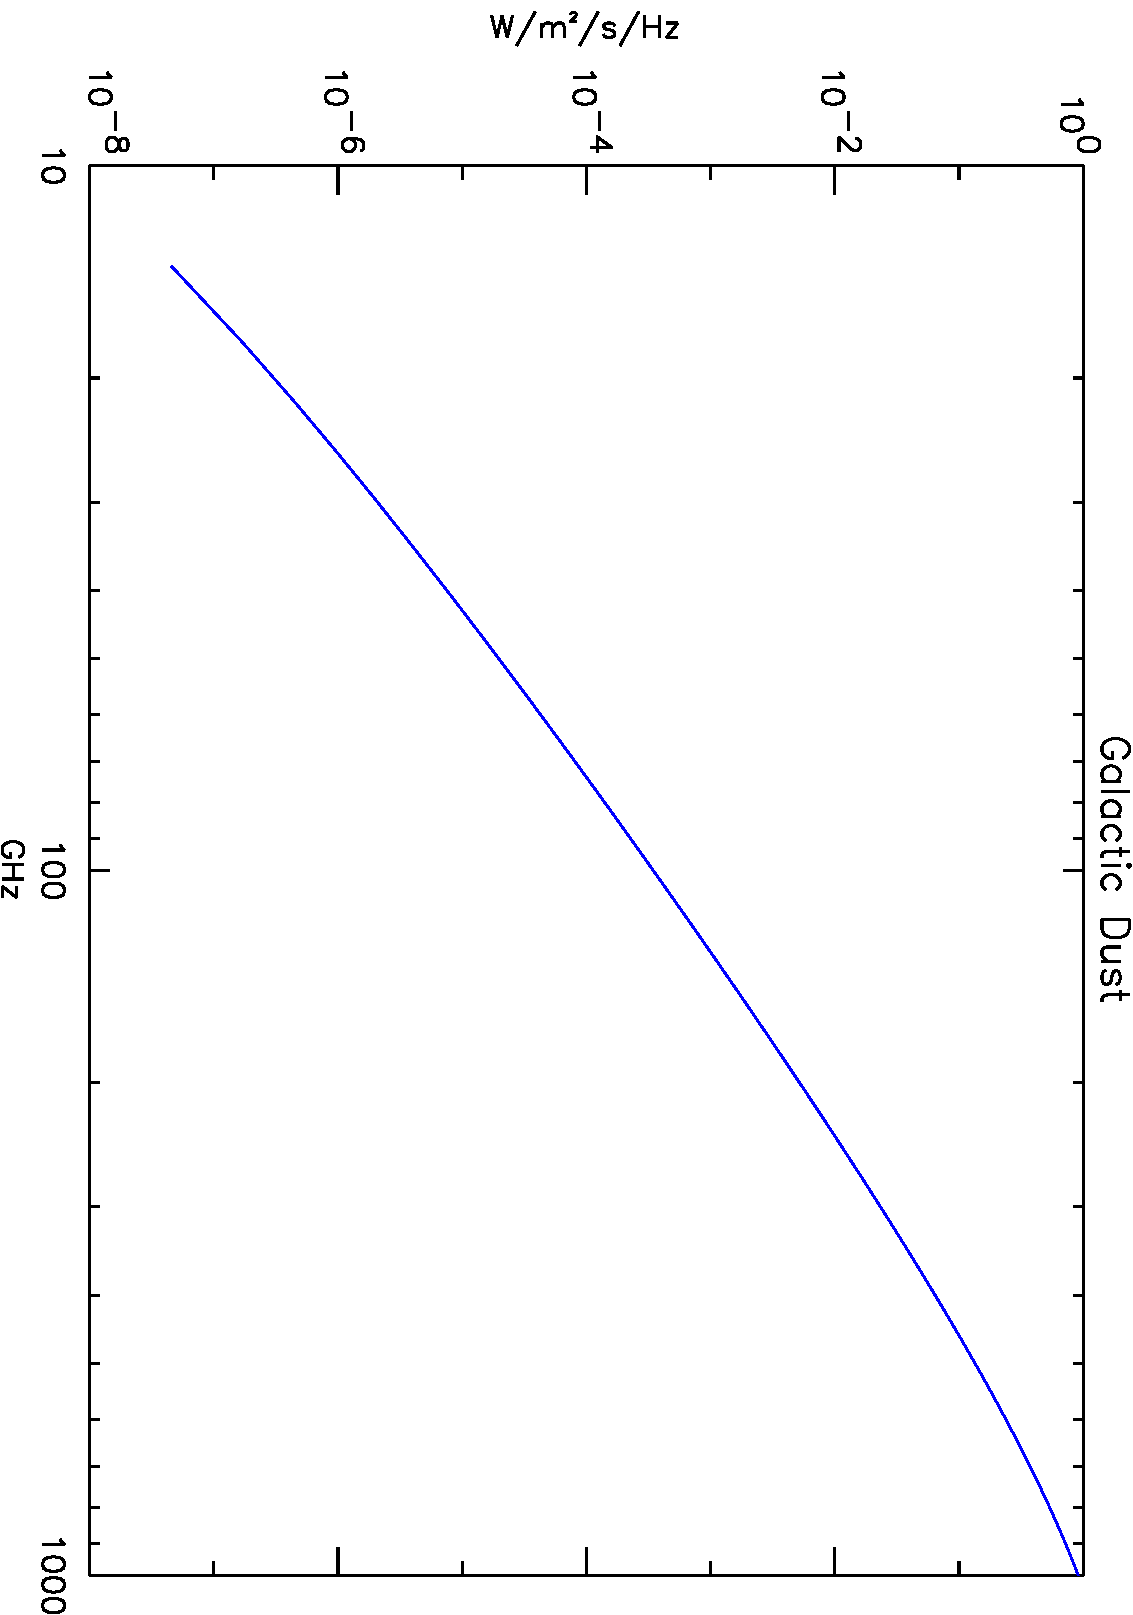
\includegraphics[angle=90,width=0.45\textwidth]{spec_gs.pdf}\hfill
    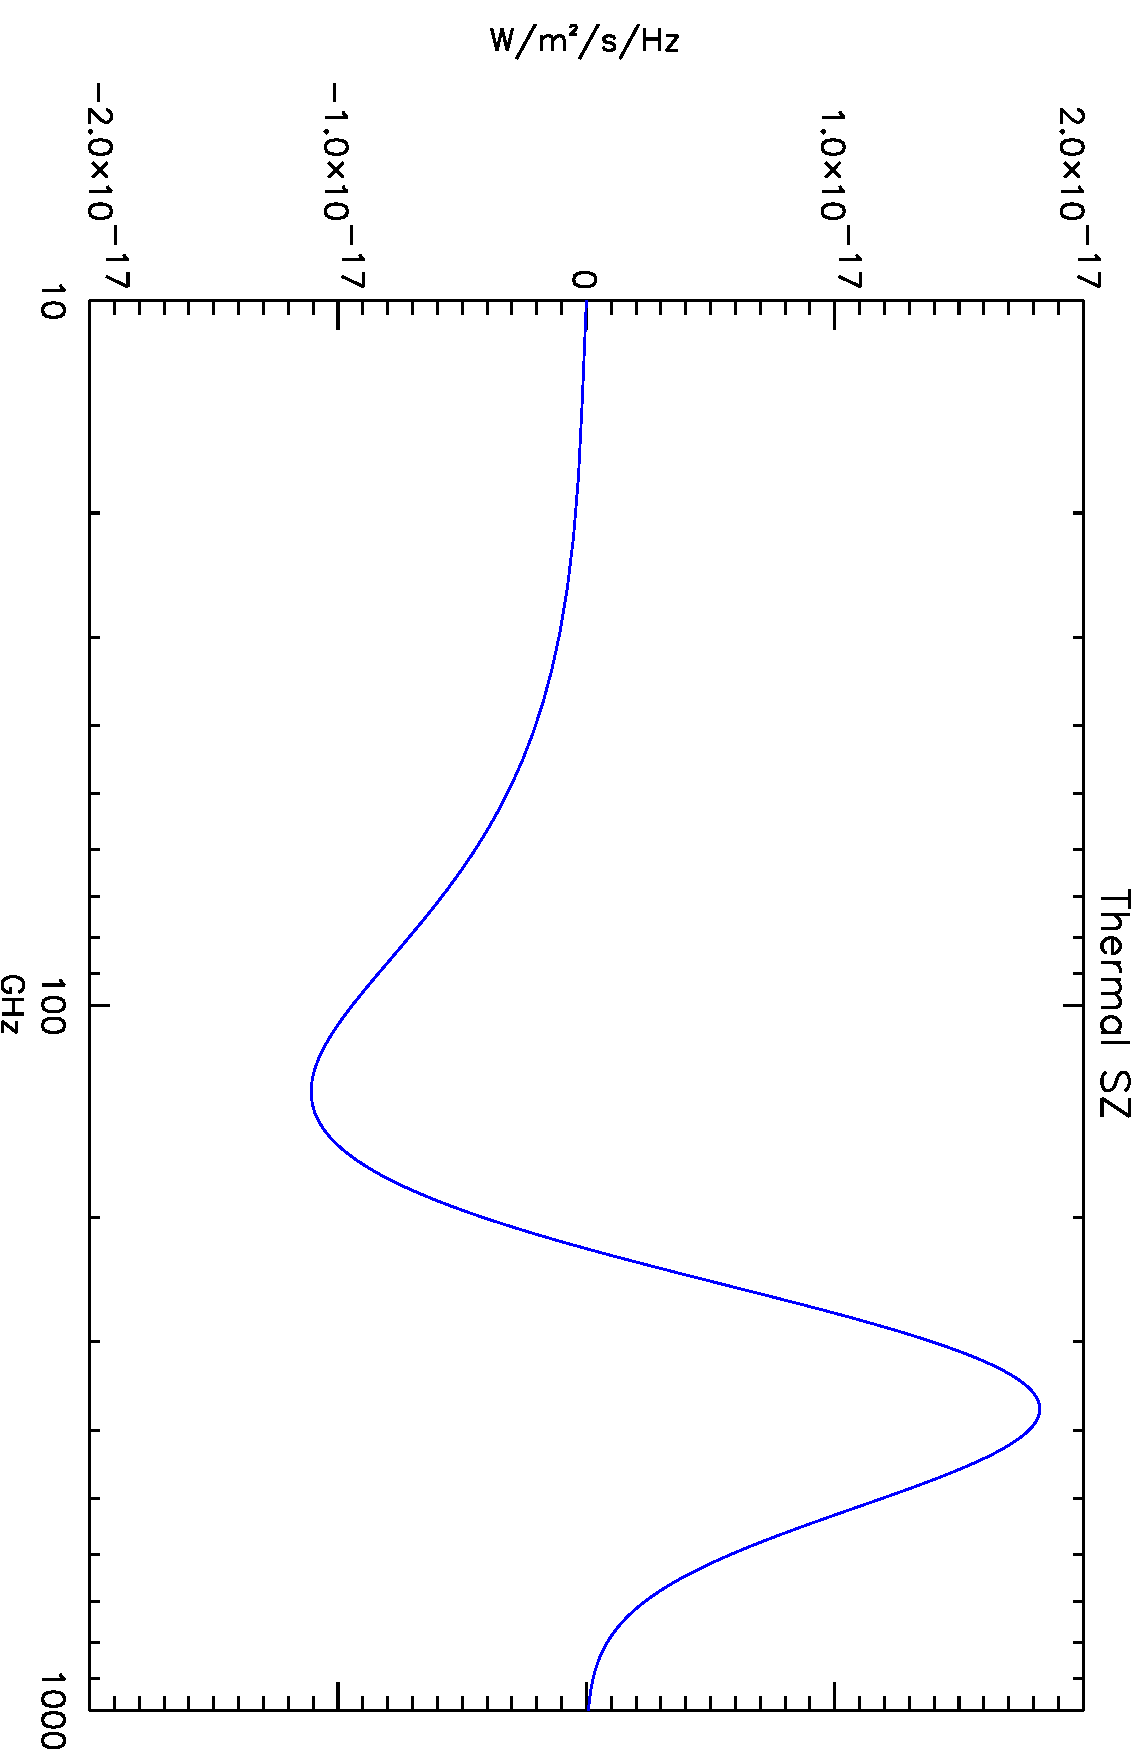
\includegraphics[angle=90,width=0.49\textwidth]{spec_sz.pdf}
  \end{center}
\caption{Spectrum for galactic dust emission (left, assumed dust temperature
  is 18K) and for the thermal SZ effect (right).\label{spec}}
\end{figure}

\begin{alltt}
almmixer [parameter file]

\input{../skymixer2/almmixer.par.txt}
\end{alltt}

\subsubsection{skymixer3}

\begin{alltt}
skymixer3 [parameter file]

\input{../skymixer2/skymixer3.par.txt}
\end{alltt}

\subsubsection {Beam}

Polarised Beam Analysis (Mark Ashdown, CPAC)

This package contains tools for reading beam data from Grasp files (in
a limited set of "cut" and "grid" sub-formats), converting polarised
beam data into Stokes parameters, calculating effective beams
including cross-polar leakage in the detectors and extracting the
spherical harmonic coefficients from the Stokes parameters.

The sources of the programs described below are commented, as are the
modules on which they are based. They are programmed in an
object-based style; data is stored in Fortran 90 types.

\begin{itemize}

\item \tw{grasp2stokes}:
Reads beam amplitudes from a Grasp file and converts them to Stokes
parameters.  This module can read three particular sub-formats of
Grasp files, called for our purposes "grd\_hfi", "grd\_lfi" and "cut".

\begin{description}
\item[grd\_hfi:] grid format file containing beam data on a polar theta-phi
	 grid.  Used by HFI for main beam simulations.  This type of
	 input will be converted into Stokes parameters on a polar
	 grid.

\item[grd\_lfi:] grid format file containing beam data on a square u-v grid.
         Used by LFI for main beam simulations.  This type of input
         will be converted into Stokes parameters on a square grid.

\item[cut:] cut format file containing beam data on constant-phi
         cuts. Usually contains full-sky data.  This type of input
         will be converted into Stokes parameters on a polar grid.
\end{description}

\begin{alltt}
grasp2stokes [parameter file]

\input{../Beam/grasp2stokes.par.txt}
\end{alltt}

\item \tw{crosspol}:
Combines two perfectly polarised beams (as produced by grasp2stokes)
to create an effective beam with detector cross-polar leakage
included.

\begin{alltt}
crosspol [parameter file]

\input{../Beam/crosspol.par.txt}
\end{alltt}

\item \tw{beam2alm}:
Reads beam Stokes parameters and then calculates their spherical
harmonic coefficients.

This program can take its input from one or two objects:

\begin{enumerate}
 \item Main beam at high resolution (the "north polar cap");
 \item Full-sky beam at lower resolution.
\end{enumerate}

Both are optional, but there must be at least one input object!

The main beam may be a polar or square beam object. If it is a square
beam object, it will be interpolated onto a polar grid before
extracting the multipoles. The full-sky beam must be in a polar beam
object.

If there is both a main beam and a full sky beam then the full sky
beam will be interpolated in the theta direction so that it has the
same theta resolution as the full sky beam. This is to give better
extraction of the multipoles.

\begin{alltt}
beam2alm [parameter file]

\input{../Beam/beam2alm.par.txt}
\end{alltt}

\item \tw{gaussbeampol}:
Calculates the multipoles of an linearly-polarised elliptical Gaussian
beam with following properties:

\begin{itemize}
  \item beam points in z-direction (towards "north pole").

  \item beam ellipse is described by three parameters:
  \begin{enumerate}
    \item mean FWHM, defined as fwhm = sqrt(fwhm\_max*fwhm\_min);
    \item ellipticity, defined as fwhm\_max/fwhm\_min;
    \item orientation angle. Major axis is oriented at angle psi\_ell to
          the x-axis;
    \item beam is polarised along direction at angle psi\_pol to the
          x-axis.
  \end{enumerate}
\end{itemize}

\begin{alltt}
gaussbeampol [parameter file]

\input{../Beam/gaussbeampol.par.txt}
\end{alltt}

\end{itemize}

\subsubsection {Total convolution}
The mathematics behind total convolution is described in Wandelt \&
G\'orski, ``Fast convolution on the sphere'', \href{http://ojps.aip.org/getpdf/servlet/GetPDFServlet?filetype=pdf&id=PRVDAQ000063000012123002000001&idtype=cvips}{Phys.~Rev.~D
  63, 123002 (2001)}, and in Challinor et al., ``All-sky convolution for
polarimetry experiments'', \href{http://ojps.aip.org/getpdf/servlet/GetPDFServlet?filetype=pdf&id=PRVDAQ000062000012123002000001&idtype=cvips}{Phys.~Rev.~D
  62, 123002 (2000)}. Briefly, the
algorithm performs full-sky convolutions of beam and sky for all
possible beam pointings, and this is repeated for all possible
rotations of the beam about its symmetry axis. The output is written
into one separate file for each beam rotation. The phrase ``all
possible'' refers to the resolution of beam and sky. If
$\ell_\mathrm{max}$ is the maximum multipole order supplied, angles on
the sphere need to be discretised into $2\ell_\mathrm{max}+1$
steps. The output per beam rotation is then written into arrays of size
$(2\ell_\mathrm{max}+1)\times(\ell_\mathrm{max}+1+\mbox{padding})$.
Likewise, if
$m_\mathrm{max}$ is the maximum multipole order describing the
azimuthal asymmetry of the beam, there are $2m_\mathrm{max}+1$
possible beam rotations.

\begin{alltt}
conviqt_v3 [parameter file]

\input{../conviqt/conviqt_v3.par.txt}
\end{alltt}

\subsubsection{simmission4}
(F.~v.~Leeuwen, D.~Mortlock, M.~Reinecke)
\label{simmission4}

    This program writes out a file containing location and pointing information
    for the Planck satellite.

    The program prepares pointing information for the Planck satellite according
    to a scanning strategy, dynamical parameters of the satellite and various
    noise estimates.

    The output consists of a file containing one record for each pointing
    period, from which it is possible to reconstruct the pointing
    of the satellite as a function of time over the pointing period to
    an accuracy level of a few arcsec.

    There is also an option to produce additional information,
    containing the results of a numerical integration over the satellite
    attitude. This produces pointing records at a requested frequency
    with an accuracy of well below one arcsec. The latter option can also
    be used to study the effects of internal torques acting on the satellite
    (such as due to moving liquids). Such effects would have to be included
    in the calculations of the torques acting on the satellite.

{\bf Note:} The samples produced by \tw{simmission4} are always evaluated at
the {\em center} of a time interval, not at its beginning! This means that
the first sample of a simulation starting at $t=0$ with a sampling rate of 1Hz
will be taken at $t=0.5$s.

\begin{alltt}
simmission4 [parameter file]

example parameter file:

\input{../simmission3/simmission4.par.txt}
\end{alltt}

\subsubsection{Focalplane}

\begin{itemize}

\item \tw{focalplane}: converts the detector database from text format to the
LevelS format.

\begin{alltt}
focalplane [parameter file]

\input{../cxxtools/focalplane.par.txt}
\end{alltt}

\end{itemize}

%---------------------------------------------------------------------
%---------------- OOF ------------------------------------------------
%---------------------------------------------------------------------

\subsubsection{OOF}

(K.~G\'orski, B.~Wandelt, C.~Burigana, D.~Maino, S.~Plaszczynski,
 M.~Reinecke)\\
This module allows the simple generation of processes
with power spectrum
\[
  P(f)=NET_\mathrm{RJ}^2\,\left[1+
      \left(\frac{f_\mathrm{knee}^{\alpha}}
               {f^{\alpha}+f_\mathrm{min}^{\alpha}}\right)
  \right]\;,
\]

where $0\leq \alpha \leq 2$.
In other words, the spectrum is white below $f_\mathrm{min}$ and above
$f_\mathrm{knee}$, and has a slope of $-\alpha$ in between. The parameters
$NET_\mathrm{RJ}$, $\alpha$, $f_\mathrm{knee}$ and $f_\mathrm{min}$ are
taken from the focal plane database.

The code contains three different implementations of the noise generator:
\begin{itemize}
  \item One algorithm is based on the superposition of a number of component
    processes, each of which is generated by evolving a set of simple
    stochastic differential equations (SDE).
  \item A fast algorithm for the special case $\alpha=2$, which uses a
    digital filter to obtain the desired spectral shape,
    was developed by S.~Plaszczynski.
  \item A still experimental algorithm nakes use of SDEs that are fed
    with one random number per sample, instead of one random number
    per SDE and per sample. Since the generation of Gaussian random numbers
    is the most time-consuming part of the code, this results in a significant
    speedup.
  \item A fast algorithm for $1<=\alpha<=2$, which uses a set of
    digital filters to obtain the desired spectral shape,
    was developed by S.~Plaszczynski. This algorithm produces noise with a
    power spectrum of
    \[P(f) = NET_\mathrm{RJ}^2 \left[ \frac{f^2+f_\mathrm{knee}^2}{f^2+f_\mathrm{min}^2} \right]^{\alpha/2}.\]
\end{itemize}

The code is not available as a stand-alone module; it is integrated into
\tw{multimod} instead.

\subsubsection{Multimod}
(R.~Hell, A.~Mennella,
 K.~G\'orski, B.~Wandelt, C.~Burigana, D.~Maino,
 M.~Bartelmann, K.~Dolag, L.~Mendes, I.~Grivell, R.~Mann,
 M.~Reinecke)

\tw{Multimod} is a C++ module which includes functionality of many modules
running after the \tw{simmission} step (i.e.\ everything dealing with
time-ordered data). Currently it includes the functionality of
\tw{detpoint}, \tw{interpol}, \tw{dipole}, \tw{oofnoise},
\tw{sampler}, \tw{countMap} and \tw{makeMap}.
The combination of various modules greatly reduces the amount of temporary
data I/O.

\begin{alltt}
multimod [parameter file]

\input{../multimod/multimod.par.txt}
\end{alltt}


%---------------------------------------------------------------------
%---------------- Tools ----------------------------------------------
%---------------------------------------------------------------------

\subsubsection{Tools}
(M. Bartelmann, MPA; M. Reinecke, MPA)

This package contains several tools to convert or modify
different types of data or provide some input data for other modules.
\begin{itemize}

\item \tw{HPXconvert\_cxx}: Convert a Healpix map between different
coordinate systems. It is used to convert foreground maps like the galactic
synchrotron map. Both unpolarised and polarised maps are supported.

\tw{HPXconvert\_cxx} operates in real space only.

\begin{verbatim}
Usage: HPXconvert_cxx <infile> <outfile> <itransform> <pol>
Transform 1: Equatorial (2000) -> Galactic   (2000)
          2: Galactic   (2000) -> Equatorial (2000)
          3: Equatorial (2000) -> Ecliptic   (2000)
          4: Ecliptic   (2000) -> Equatorial (2000)
          5: Ecliptic   (2000) -> Galactic   (2000)
          6: Galactic   (2000) -> Ecliptic   (2000)
          7: Equatorial (1950) -> Galactic   (1950)
          8: Galactic   (1950) -> Equatorial (1950)
          9: Equatorial (1950) -> Ecliptic   (1950)
         10: Ecliptic   (1950) -> Equatorial (1950)
         11: Ecliptic   (1950) -> Galactic   (1950)
         12: Galactic   (1950) -> Ecliptic   (1950)

pol: T or F
\end{verbatim}

\item \tw{rotmap\_cxx}: Convert a Healpix map between different
coordinate systems. It is used to convert foreground maps like the galactic
synchrotron map. Both unpolarised and polarised maps are supported.
The rotation algorithm used in this code is different from
\tw{HPXconvert\_cxx} and works as follows:
\begin{itemize}
  \item extract $a_{lm}$ from the input map, using an iterative scheme
        with 3 iterations, up to $l_{\mbox{max}}=3N_{\mbox{side}}$
  \item perform the rotation in $a_{lm}$ space
  \item convert the rotated $a_{lm}$ back to a HEALPix map
\end{itemize}
This code is rather resource-consuming, but much more accurate than
\tw{HPXconvert\_cxx}.

\begin{verbatim}
Usage: rotmap_cxx <infile> <outfile> <itransform> <pol>
Transform 1: Equatorial (2000) -> Galactic   (2000)
          2: Galactic   (2000) -> Equatorial (2000)
          3: Equatorial (2000) -> Ecliptic   (2000)
          4: Ecliptic   (2000) -> Equatorial (2000)
          5: Ecliptic   (2000) -> Galactic   (2000)
          6: Galactic   (2000) -> Ecliptic   (2000)
          7: Equatorial (1950) -> Galactic   (1950)
          8: Galactic   (1950) -> Equatorial (1950)
          9: Equatorial (1950) -> Ecliptic   (1950)
         10: Ecliptic   (1950) -> Equatorial (1950)
         11: Ecliptic   (1950) -> Galactic   (1950)
         12: Galactic   (1950) -> Ecliptic   (1950)

pol: T or F
\end{verbatim}

\item \tw{rotalm\_cxx}: Converts $a_{lm}$ between different
coordinate systems.

\begin{verbatim}
Usage: rotalm_cxx <infile> <outfile> <itransform> <pol>
Transform 1: Equatorial (2000) -> Galactic   (2000)
          2: Galactic   (2000) -> Equatorial (2000)
          3: Equatorial (2000) -> Ecliptic   (2000)
          4: Ecliptic   (2000) -> Equatorial (2000)
          5: Ecliptic   (2000) -> Galactic   (2000)
          6: Galactic   (2000) -> Ecliptic   (2000)
          7: Equatorial (1950) -> Galactic   (1950)
          8: Galactic   (1950) -> Equatorial (1950)
          9: Equatorial (1950) -> Ecliptic   (1950)
         10: Ecliptic   (1950) -> Equatorial (1950)
         11: Ecliptic   (1950) -> Galactic   (1950)
         12: Galactic   (1950) -> Ecliptic   (1950)

pol: T or F
\end{verbatim}

\item \tw{fpdbhelper}: Command-line tool to retrieve data from the focal plane
database. Mainly intended for automatic parameter file generation.

\begin{verbatim}
Usage: fpdbhelper <database> <detector> <quantity>

<database>: name of the focalplane data base file

<detector>: name of the required detector

<quantity>: determines the output of the program
  fwhm_arcmin   : FWHM in arc minutes
  freq_GHz      : central frequency in GHz
                  (rounded to the nearest integer)
  lmax          : a hint at a suitable lmax parameter for this detector
  ringres       : number of samples taken per minute
                  (rounded to the nearest integer)
  f_samp        : sampling frequency (in Hz)
  alpha         : slope of the noise spectrum (as a positive number)
  f_knee        : knee frequency (in Hz)
  f_min         : minimum noise frequency (in Hz)
  net_rj        : noise equivalent antenna temperature (in K/sqrt(Hz))
  tau_bol       : bolometer time constant (in s)
  tau_int       : integration time for each sample (in s)
  ellipticity   : (max FWHM)/(min FWHM)
  theta_uv_deg  : the theta_uv angle (in degrees)
  phi_uv_deg    : the phi_uv angle (in degrees)
  psi_uv_deg    : the psi_uv angle (in degrees)
  psi_pol_deg   : the psi_pol angle (in degrees)
  psi_ell_deg   : the psi_ell angle (in degrees)
\end{verbatim}

\item \tw{makeMap}: Makes a map out of sampled detector pointings
and \tw{TOD}.

\begin{alltt}
makeMap [TOD] [DETPNT] [baseoutname] [RES]
\end{alltt}


\item \tw{addTOI}:
(Davide Maino, Martin Reinecke) Coadd a number of different \tw{TOI}.

\begin{alltt}
\input{../cxxtools/addTOI.par.txt}
\end{alltt}

\item \tw{addMaps}:
(Davide Maino, Martin Reinecke) Coadd a number of different Healpix maps.

\begin{alltt}
\input{../cxxtools/addMaps.par.txt}
\end{alltt}

\item \tw{beamsampler}:
(Martin Reinecke) Smear a set of beam $a_{lm}$ to simulate the effect
of the detector electronics.

\begin{alltt}
\input{../cxxtools/beamsampler.par.txt}
\end{alltt}

\item \tw{sat2quat}:
(Martin Reinecke) Converts the detailed satellite pointings produced by
\tw{simmission} to quaternions.

\begin{alltt}
\input{../cxxtools/sat2quat.par.txt}
\end{alltt}

\item \tw{pointing\_errors}:
(Martin Reinecke) Adds random perturbations to satellite pointing quaternions.

\begin{alltt}
\input{../cxxtools/pointing_errors.par.txt}
\end{alltt}

\item \tw{gapmaker}:
(Martin Reinecke) Introduces gaps into time-ordered information produced
by \tw{multimod}; this can be done either by cutting out data (for LFI) or
flagging data as non-existent (for HFI).

\begin{alltt}
\input{../multimod/gapmaker.par.txt}
\end{alltt}

\item \tw{mult\_alm}:
(Martin Reinecke) Allows convolution and deconvolution of $a_{lm}$ with
Gaussian beams and/or pixel window functions.

\begin{alltt}
\input{../Healpix_cxx/mult_alm.par.txt}
\end{alltt}

\end{itemize}

\subsubsection{LFI-specific modules}

\begin{itemize}
\item \tw{ls2lfitoi} (D.~Maino, UniMI):

\tw{ls2lfitoi} is a C++ module which produces un-differenced data
(i.e.\ sky and load signals) according to LFI DDL.

\begin{alltt}
ls2lfitoi [parameter file]
\end{alltt}
\verbatiminput {../LFI-specific/ls2lfitoi.par.txt}

The way in which Sky and Load data are constructed has been subject
of discussion within the LFI-Demo group. Here is the algorithm as
it is implemented now.

First of all one defined the ``target'' value of the gain modulation
factor $R$ parameter as
\begin{equation}
R_{\rm target} = \frac{\langle T_{\rm sky}\rangle
                 + T_{\rm noise}}{T_{\rm load} + T_{\rm noise}}\, .
\end{equation}
Once this is done one constructs the signal from Sky and Load with the
following expressions:
\begin{eqnarray}
V_{\rm sky} = {\rm signal TOI} + T_{0,CMB} + \frac{\rm wn1}{\sqrt{2}}
            + {\rm ooftp} + {\rm oof/2} + T_{\rm noise}\\
V_{\rm load} = T_{\rm load} + \frac{\rm wn2}{\sqrt{2}} +
             \frac{{\rm ooftp - oof/2}}{R_{\rm target}} + T_{\rm noise}
\end{eqnarray}

One would like to derive the value of the $R$ parameter in order
to construct the differenced data usually taking the ratio of the mean
values of $V_{\rm sky}$ and $V_{\rm load}$
on suitable time lag and then build the quantity
$V_{\rm sky} - R_{\rm estimated} V_{\rm load}$. With
the actual recipe this quantity contains the correct value of the
signal, the correct amount of white noise and only the differenced part
of $1/f$ noise since the total power part is suppressed by
a factor proportional to the difference between the target and the
estimated value of $R$.

\item \tw{quantum} (Michele Maris, OAT, and Davide Maino, UniMI):

\tw{quantum} is a C++ module which simulates the on-board
processing of PType 2 data and the subsequent decoding and
conversion to TOI in the DPC L1. In particular it
simulates the activity of PType 2 processing from PType 1 data.
The code accepts data in input of toi.science.Data type specified in
the LFI DDL (and built-in into the delivered DDL with LevelS from
ESTEC CVS). It is able to reproduce the creation of two sets of
differenced data with two different and known value
of the gain modulation factors (gmf1 and gmf2). This is
done in order to satisfy the constraints related to transmission
band-width from S/C to ground station.

\begin{alltt}
quantum [parameter file]
\end{alltt}
\verbatiminput {../LFI-specific/quantum.par.txt}

\item \tw{ahf2satpt} (Martin Reinecke, MPA):

This module reads a set of AHF objects with the DDL type
\tw{toi.attitude.HighFrequency}, extracts the satellite pointing information
from these and writes it into a single new object of type
\tw{sat.LS\_satpoint\_real}.
This object contains a list of all input satellite quaternions and their time
stamps, as well as a list of name, start time, end time, index of the first
quaternion and total number of quaternions for every pointing period found in
the input AHFs.

\begin{alltt}
ahf2satpt [parameter file]
\end{alltt}
\verbatiminput {../LFI-specific/ahf2satpt.par.txt}
\end{itemize}


\appendix

\clearpage
\section{LevelS dataflow}
\begin{figure}[h]
  \begin{center}
    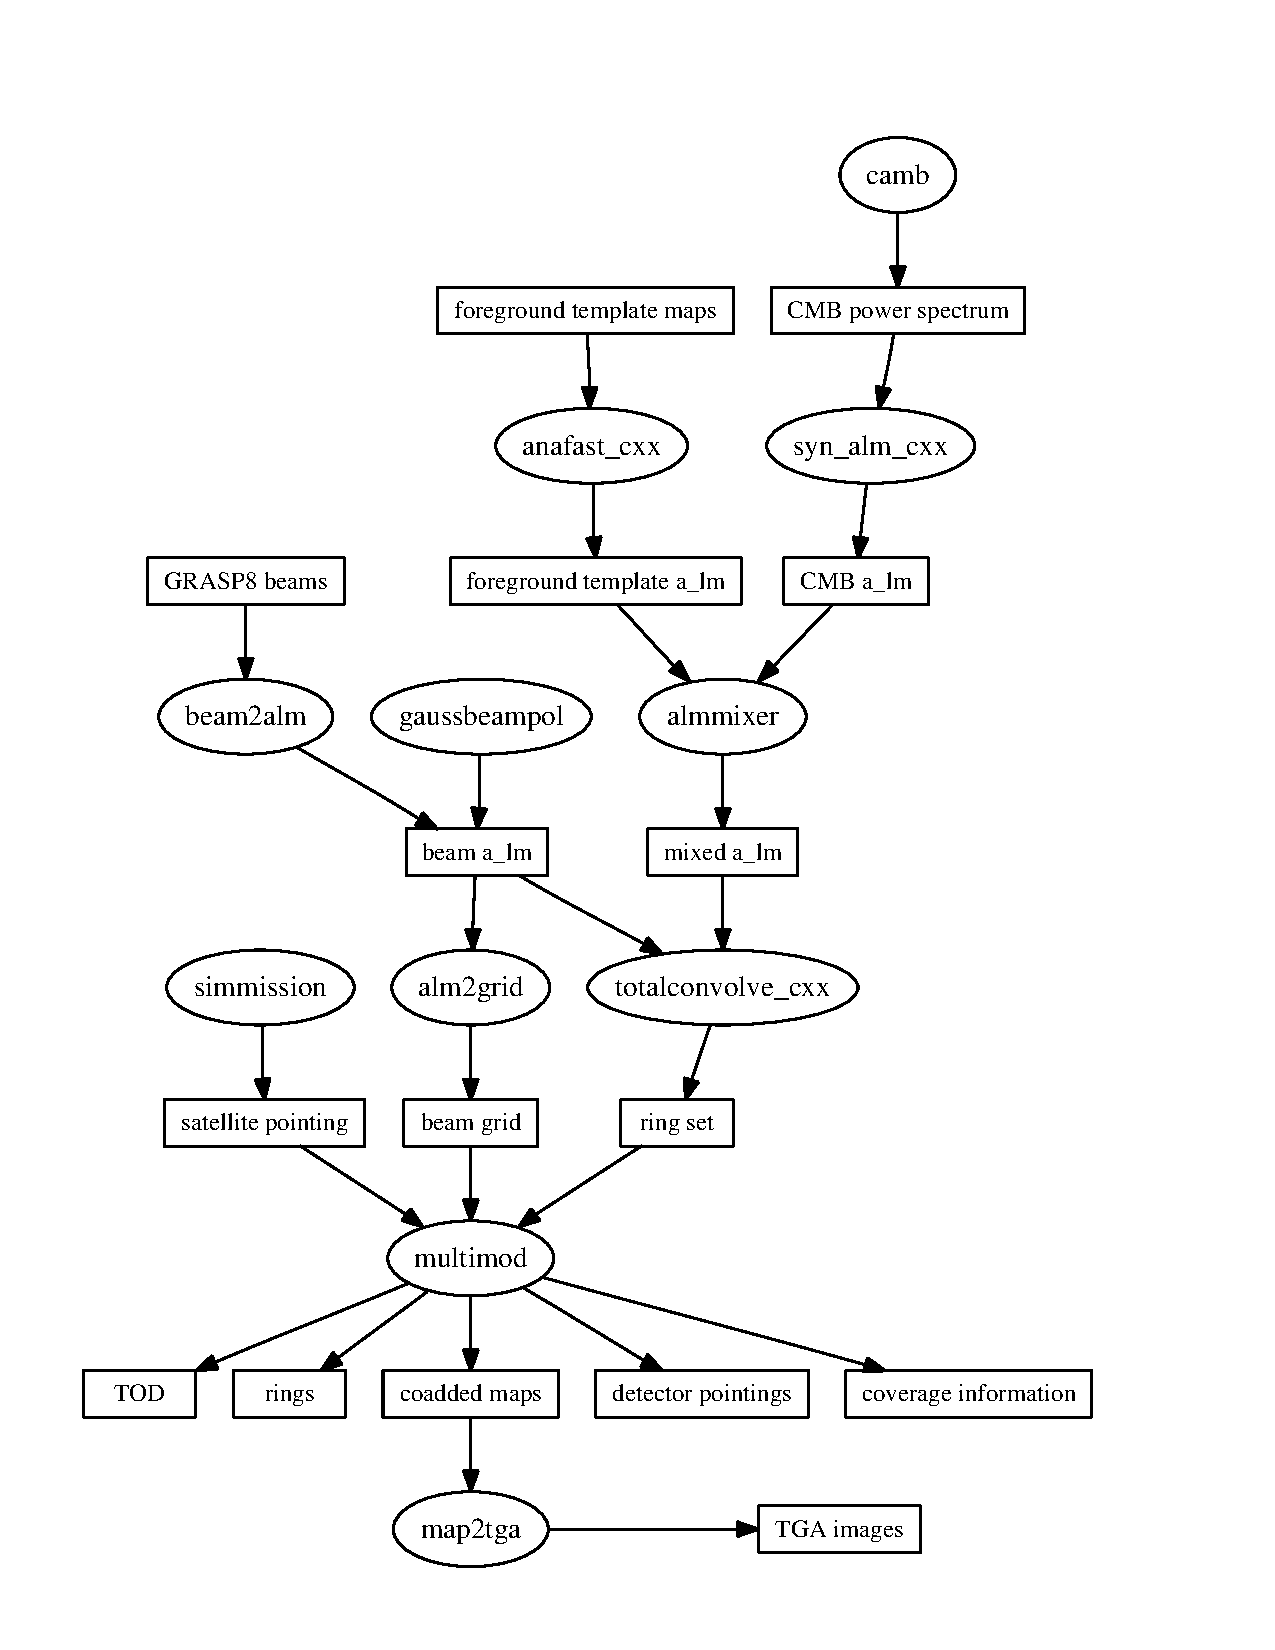
\includegraphics[angle=0,height=0.8\textheight]{pipeline.pdf}
  \end{center}
  \caption{Schematic dataflow of a typical \emph{Planck} simulation pipeline.
  Rectangular components denote data products, whereas elliptic
  shapes represent modules.}
\end{figure}

\clearpage
\section{Detector Database}

For reference, we reproduce here the detector database:
{\tiny
\begin{alltt}
\input{../cxxtools/fp_database.txt}
\end{alltt}}


\end{document}
